% Important: If latex complains about unicode characters,
% please use "\usepackage[utf8x]{inputenc}" in your preamble
% You can change the size of the picture by putting it into the construct:
% 1) \resizebox{10cm}{!}{"below picture"} to scale horizontally to 10 cm
% 2) \resizebox{!}{15cm}{"below picture"} to scale vertically to 15 cm
% 3) \resizebox{10cm}{15cm}{"below picture"} a combination of above two
% It is not recomended to use the scale option of the tikzpicture environment.
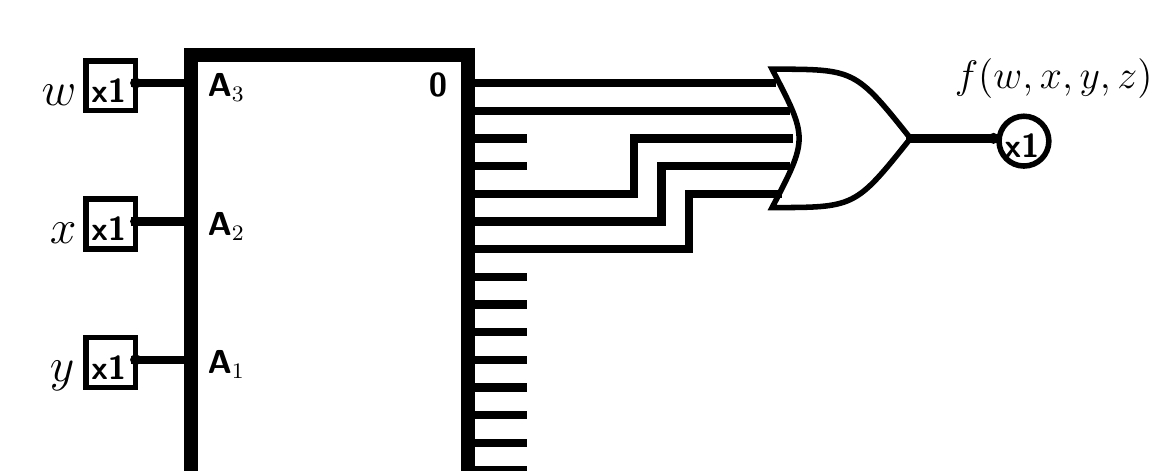
\begin{tikzpicture}[x=1pt,y=-1pt,line cap=rect]
\useasboundingbox (0,0) rectangle (400,150);
\definecolor{custcol_0_0_0}{RGB}{0, 0, 0}
\definecolor{custcol_ff_ff_ff}{RGB}{255, 255, 255}
\draw [line width=3.0pt, custcol_0_0_0 ]  (319.0,40.0) -- (349.0,40.0) ;
\draw [line width=3.0pt, custcol_0_0_0 ]  (159.0,130.0) -- (179.0,130.0) ;
\draw [line width=3.0pt, custcol_0_0_0 ]  (159.0,90.0) -- (179.0,90.0) ;
\draw [line width=3.0pt, custcol_0_0_0 ]  (159.0,40.0) -- (179.0,40.0) ;
\draw [line width=3.0pt, custcol_0_0_0 ]  (159.0,50.0) -- (179.0,50.0) ;
\draw [line width=3.0pt, custcol_0_0_0 ]  (159.0,100.0) -- (179.0,100.0) ;
\draw [line width=3.0pt, custcol_0_0_0 ]  (159.0,110.0) -- (179.0,110.0) ;
\draw [line width=3.0pt, custcol_0_0_0 ]  (159.0,120.0) -- (179.0,120.0) ;
\draw [line width=3.0pt, custcol_0_0_0 ]  (159.0,140.0) -- (179.0,140.0) ;
\draw [line width=3.0pt, custcol_0_0_0 ]  (159.0,150.0) -- (179.0,150.0) ;
\draw [line width=3.0pt, custcol_0_0_0 ]  (159.0,160.0) -- (179.0,160.0) ;
\draw [line width=3.0pt, custcol_0_0_0 ]  (159.0,170.0) -- (179.0,170.0) ;
\draw [line width=3.0pt, custcol_0_0_0 ]  (39.0,20.0) -- (59.0,20.0) ;
\draw [line width=3.0pt, custcol_0_0_0 ]  (39.0,70.0) -- (59.0,70.0) ;
\draw [line width=3.0pt, custcol_0_0_0 ]  (39.0,120.0) -- (59.0,120.0) ;
\draw [line width=3.0pt, custcol_0_0_0 ]  (39.0,170.0) -- (59.0,170.0) ;
\draw [line width=5.0pt, custcol_0_0_0 ]  (59.0,10.0) -- (158.0,10.0) ;
\draw [line width=5.0pt, custcol_0_0_0 ]  (159.0,10.0) -- (159.0,179.0) ;
\draw [line width=5.0pt, custcol_0_0_0 ]  (159.0,180.0) -- (60.0,180.0) ;
\draw [line width=5.0pt, custcol_0_0_0 ]  (59.0,180.0) -- (59.0,11.0) ;
\fontsize{12pt}{12pt}\fontseries{bx}\sffamily\selectfont\node[inner sep=0, outer sep=0, custcol_0_0_0, anchor=base west] at  (145.0,25.0)  {0};
\fontsize{12pt}{12pt}\fontseries{bx}\sffamily\selectfont\node[inner sep=0, outer sep=0, custcol_0_0_0, anchor=base west] at  (65.0,125.0)  {A$_1$};
\fontsize{12pt}{12pt}\fontseries{bx}\sffamily\selectfont\node[inner sep=0, outer sep=0, custcol_0_0_0, anchor=base west] at  (65.0,175.0)  {A$_0$};
\fontsize{12pt}{12pt}\fontseries{bx}\sffamily\selectfont\node[inner sep=0, outer sep=0, custcol_0_0_0, anchor=base west] at  (65.0,75.0)  {A$_2$};
\fontsize{12pt}{12pt}\fontseries{bx}\sffamily\selectfont\node[inner sep=0, outer sep=0, custcol_0_0_0, anchor=base west] at  (65.0,25.0)  {A$_3$};
\fill [line width=1.0pt, custcol_0_0_0]  (59.0,20.0) ellipse (2.0 and 2.0 );
\fill [line width=1.0pt, custcol_0_0_0]  (59.0,70.0) ellipse (2.0 and 2.0 );
\fill [line width=1.0pt, custcol_0_0_0]  (59.0,120.0) ellipse (2.0 and 2.0 );
\fill [line width=1.0pt, custcol_0_0_0]  (59.0,170.0) ellipse (2.0 and 2.0 );
\fill [line width=1.0pt, custcol_0_0_0]  (159.0,20.0) ellipse (2.0 and 2.0 );
\fill [line width=1.0pt, custcol_0_0_0]  (159.0,30.0) ellipse (2.0 and 2.0 );
\fill [line width=1.0pt, custcol_0_0_0]  (159.0,40.0) ellipse (2.0 and 2.0 );
\fill [line width=1.0pt, custcol_0_0_0]  (159.0,50.0) ellipse (2.0 and 2.0 );
\fill [line width=1.0pt, custcol_0_0_0]  (159.0,60.0) ellipse (2.0 and 2.0 );
\fill [line width=1.0pt, custcol_0_0_0]  (159.0,70.0) ellipse (2.0 and 2.0 );
\fill [line width=1.0pt, custcol_0_0_0]  (159.0,80.0) ellipse (2.0 and 2.0 );
\fill [line width=1.0pt, custcol_0_0_0]  (159.0,90.0) ellipse (2.0 and 2.0 );
\fill [line width=1.0pt, custcol_0_0_0]  (159.0,100.0) ellipse (2.0 and 2.0 );
\fill [line width=1.0pt, custcol_0_0_0]  (159.0,110.0) ellipse (2.0 and 2.0 );
\fill [line width=1.0pt, custcol_0_0_0]  (159.0,120.0) ellipse (2.0 and 2.0 );
\fill [line width=1.0pt, custcol_0_0_0]  (159.0,130.0) ellipse (2.0 and 2.0 );
\fill [line width=1.0pt, custcol_0_0_0]  (159.0,140.0) ellipse (2.0 and 2.0 );
\fill [line width=1.0pt, custcol_0_0_0]  (159.0,150.0) ellipse (2.0 and 2.0 );
\fill [line width=1.0pt, custcol_0_0_0]  (159.0,160.0) ellipse (2.0 and 2.0 );
\fill [line width=1.0pt, custcol_0_0_0]  (159.0,170.0) ellipse (2.0 and 2.0 );
\draw [line width=2.0pt, custcol_0_0_0 ]  (21.0,12.0) -- (38.0,12.0) ;
\draw [line width=2.0pt, custcol_0_0_0 ]  (39.0,12.0) -- (39.0,29.0) ;
\draw [line width=2.0pt, custcol_0_0_0 ]  (39.0,30.0) -- (22.0,30.0) ;
\draw [line width=2.0pt, custcol_0_0_0 ]  (21.0,30.0) -- (21.0,13.0) ;
\fontsize{12pt}{12pt}\selectfont\node[inner sep=0, outer sep=0, custcol_0_0_0, anchor=base west] at  (23.0,27.0)  {x1};
\fontsize{16pt}{16pt}\fontseries{bx}\selectfont\node[inner sep=0, outer sep=0, custcol_0_0_0, anchor=base west] at  (5.0,28.0)  {$w$};
\fill [line width=2.0pt, custcol_0_0_0]  (39.0,20.0) ellipse (2.0 and 2.0 );
\draw [line width=2.0pt, custcol_0_0_0 ]  (21.0,62.0) -- (38.0,62.0) ;
\draw [line width=2.0pt, custcol_0_0_0 ]  (39.0,62.0) -- (39.0,79.0) ;
\draw [line width=2.0pt, custcol_0_0_0 ]  (39.0,80.0) -- (22.0,80.0) ;
\draw [line width=2.0pt, custcol_0_0_0 ]  (21.0,80.0) -- (21.0,63.0) ;
\fontsize{12pt}{12pt}\selectfont\node[inner sep=0, outer sep=0, custcol_0_0_0, anchor=base west] at  (23.0,77.0)  {x1};
\fontsize{16pt}{16pt}\fontseries{bx}\selectfont\node[inner sep=0, outer sep=0, custcol_0_0_0, anchor=base west] at  (8.0,78.0)  {$x$};
\fill [line width=2.0pt, custcol_0_0_0]  (39.0,70.0) ellipse (2.0 and 2.0 );
\draw [line width=2.0pt, custcol_0_0_0 ]  (21.0,112.0) -- (38.0,112.0) ;
\draw [line width=2.0pt, custcol_0_0_0 ]  (39.0,112.0) -- (39.0,129.0) ;
\draw [line width=2.0pt, custcol_0_0_0 ]  (39.0,130.0) -- (22.0,130.0) ;
\draw [line width=2.0pt, custcol_0_0_0 ]  (21.0,130.0) -- (21.0,113.0) ;
\fontsize{12pt}{12pt}\selectfont\node[inner sep=0, outer sep=0, custcol_0_0_0, anchor=base west] at  (23.0,127.0)  {x1};
\fontsize{16pt}{16pt}\fontseries{bx}\selectfont\node[inner sep=0, outer sep=0, custcol_0_0_0, anchor=base west] at  (8.0,128.0)  {$y$};
\fill [line width=2.0pt, custcol_0_0_0]  (39.0,120.0) ellipse (2.0 and 2.0 );
\draw [line width=2.0pt, custcol_0_0_0 ]  (21.0,162.0) -- (38.0,162.0) ;
\draw [line width=2.0pt, custcol_0_0_0 ]  (39.0,162.0) -- (39.0,179.0) ;
\draw [line width=2.0pt, custcol_0_0_0 ]  (39.0,180.0) -- (22.0,180.0) ;
\draw [line width=2.0pt, custcol_0_0_0 ]  (21.0,180.0) -- (21.0,163.0) ;
\fontsize{12pt}{12pt}\selectfont\node[inner sep=0, outer sep=0, custcol_0_0_0, anchor=base west] at  (23.0,177.0)  {x1};
\fontsize{16pt}{16pt}\fontseries{bx}\selectfont\node[inner sep=0, outer sep=0, custcol_0_0_0, anchor=base west] at  (9.0,178.0)  {$z$};
\fill [line width=2.0pt, custcol_0_0_0]  (39.0,170.0) ellipse (2.0 and 2.0 );
\draw [line width=3.0pt, custcol_0_0_0 ]  (159.0,20.0) -- (269.0,20.0) -- (269.0,20.0) ;
\draw [line width=3.0pt, custcol_0_0_0 ]  (159.0,30.0) -- (269.0,30.0) -- (274.0,30.0) ;
\draw [line width=3.0pt, custcol_0_0_0 ]  (159.0,60.0) -- (219.0,60.0) -- (219.0,40.0) -- (269.0,40.0) -- (275.0,40.0) ;
\draw [line width=3.0pt, custcol_0_0_0 ]  (159.0,70.0) -- (229.0,70.0) -- (229.0,50.0) -- (269.0,50.0) -- (274.0,50.0) ;
\draw [line width=3.0pt, custcol_0_0_0 ]  (159.0,80.0) -- (239.0,80.0) -- (239.0,60.0) -- (269.0,60.0) -- (271.0,60.0) ;
\draw [line width=2.0pt, custcol_0_0_0 ]  (319.0,40.0) .. controls  (299.0,15.0)  ..  (269.0,15.0) .. controls  (282.0,40.0)  ..  (269.0,65.0) .. controls  (299.0,65.0)  ..  (319.0,40.0) -- cycle ;
\draw [line width=2.0pt, custcol_0_0_0]  (360.0,41.0) ellipse (9.0 and 9.0 );
\fontsize{12pt}{12pt}\selectfont\node[inner sep=0, outer sep=0, custcol_0_0_0, anchor=base west] at  (353.0,47.0)  {x1};
\fill [line width=2.0pt, custcol_0_0_0]  (349.0,40.0) ellipse (2.0 and 2.0 );
\fontsize{14pt}{14pt}\selectfont\node[inner sep=0, outer sep=0, custcol_0_0_0, anchor=base west] at  (335.0,22.0)  {$f(w,x,y,z)$};
\end{tikzpicture}

